%%%%%%%%%%%%%%%%%%%%%%%%%%%%%%%%%%%%%%%%%%%%%%%%%%%%%%%%%%%%%%%%%%%%%%%%%%%%%%%%
%%%%%%%%%%%%%%%%%%%%%%%%%%%%%%%%%%%%%%%%%%%%%%%%%%%%%%%%%%%%%%%%%%%%%%%%%%%%%%%%
%% Chapter - Introduction
%%%%%%%%%%%%%%%%%%%%%%%%%%%%%%%%%%%%%%%%%%%%%%%%%%%%%%%%%%%%%%%%%%%%%%%%%%%%%%%%
%%%%%%%%%%%%%%%%%%%%%%%%%%%%%%%%%%%%%%%%%%%%%%%%%%%%%%%%%%%%%%%%%%%%%%%%%%%%%%%%

\startfirstchapter{Introduction}
\label{chap:introduction}

In recent years, advances in computerized recording, storage and
processing technology have enabled bioacoustic researchers to collect,
digitize and store very large archives of bioacoustic data from a wide
variety of species. The size and number of these large bioacoustic
archives is growing rapidly, and the creation of tools to help
researchers in bioacoustics make sense of this data is an area of
ongoing research \cite{halkias2013icml4b}.

Concurrently in the field of Computer Science, advances in audio
feature extraction and machine learning have made it possible to
extract meaning from raw audio as is shown by the successes of the
field of Music Information Retrieval \cite{tzanetakis2008marsyas}.  In
our lab, we are interested in studying these large bioacoustic
archives with new audio feature extraction and machine learning
algorithms.  However, for each of these large bioacoustic archives,
considerable knowledge of the vocalizations of the species represented
in the archives is required.  For example, in order to annotate a
field recording of bird songs, knowledge of the different
vocalizations of each of the birds present is required, and experts in
birds vocalizations from one region might not be experts in another
region.  In addition, the rapid pace of development of audio feature
extraction and machine learning algorithms would require a computer
science expert to apply them.

What is required is some way for computer scientists and biologists to
collaborate so that the extensive biological knowledge of the
biologists can be combined with the tools and knowledge of computer
scientists to study large bioacoustic archives.  Many successful
examples of this collaboration have occurred in the past with smaller
datasets \cite{yurkphd}, with biologists using tools such as Raven
\cite{cornell2011raven} to annotate recordings, and then using audio
feature extraction and machine learning algorithms
\cite{deecke1999quantifying} or collaborating with computer scientists
to extract information from these recordings.

The vast size of the new bioacoustic archives presents challenges for
these traditional tools based on a single computer model of
computation and designed to work on individual sound recordings rather
than collections of them. The first problem is simply the vast size of
these audio collections.  With a dataset in the range of tens of
thousands of hours \cite{ness2013orchive} to hundreds of thousands of
hours \cite{urazghildiiev2009rightwhale}, it would be impractical for
each computer to have its own copy of the data.  Furthermore, it would
take an impractical amount of time to extract audio features and use
machine learning on these datasets on a single computer.

For many of these sources of bioacoustic data, there are only few
experts that are capable of annotating this data, and because they
often spend considerable time in the field, the time they have to
annotate recordings is very limited.  It should also be noted that the
biologists who have the most knowledge of the vocalizations of the
species of interest are often not directly working on the same
bioacoustic data mining project that the computer scientists are
working on and would only indirectly obtain benefits from doing the
large number of annotations that are required.  In some cases, such as
the right whale project from Cornell Lab of Ornithology Bioacoustics
Research Program or the Alberta Biodiversity Monitoring Institute,
biologists are hired specifically to annotate recordings.  In the case
of the Orchive, most of the annotations were generously volunteered by
biologists working on other projects, and the labels did not directly
benefit their research.  It was difficult to obtain annotations from
more experienced orca researchers simply because they were very busy
on their own research projects.

However, some of the subjects of bioacoustic archives are quite
charismatic species, such as whales, dolphins, birds and frogs, and
there are many members of the public that already listen to recordings
of these species for pleasure \footnote{\url{http://orca-live.net}}
\footnote{\url{http://http://birdsong.fm/}} There already exist
systems for enabling these members of the public to be citizen
scientists \cite{anze08galaxyzoo} and to help scientists by annotating
data \cite{taylor2009neptune}.  These member of the public are engaged
and with some training can be citizen scientists and help biologists
by annotating data.

In this thesis, a system is developed and presented to help biologists
and computer scientists collaborate on the annotation, segmentation
and classification of large bioacoustic archives.  It uses web-based
technology to allow groups of biologists to listen to, view, and
annotate recordings, and enables computer scientists to extract audio
features from these recordings and to use the annotations by
biologists to train machine learning systems.  This software also has
the functionality to display the output of the audio feature
extraction and machine learning algorithms in a form that both the
biologists and computer scientists can easily use.  In addition, it
provides a serious casual game interface that allows citizen
scientists to help annotate data, and allows both the biologists and
computer scientists to use these annotations to derive knowledge from
the archive.

Because this system involves many different people interacting with it
at many different times and places, it is amenable to study by
Distributed Cognition \cite{hutchins1996cognition}, a field that
acknowledges the importance of the social and physical environment on
the system under study.  It also has drawn ideas and inspiration from
the field of Computer Supported Collaborative Work (CSCW)
\cite{bannon1991cscw} where computers are used to help groups of
people work together more effectively.  In order to train the machine
learning system to segment the recordings into clips and then to
classify these call types, this system must get input by at least two very
different communities, developers of bioacoustic algorithms and
biologists trained to be experts in orca vocalizations, with perhaps
additional contributions by citizen scientists.  Co-ordinating work
between these communities will be difficult, and determining who needs
what data and who has to do what work in order to get that
data\cite{grudin1988cscw} will be of primary importance if this
project is to succeed.  An early hypothesis that was employed for most
of this project was that the experts in orca vocalizations would both
do the work and also would get the rewards.  This hypothesis will be
examined later in the thesis.

The ultimate goal of the use of this system is to take a large
unannotated bioacoustic archive and to segment and annotate it using a
combination of expert knowledge, annotations from citizen scientists
and to take these labels and classify its audio features using machine
learning systems.  The system I present will use data from the
Orchive, a large collection of over \aboutNumberOfOrchiveRecordings
hours of orca vocalizations collected over the last
\totalYearsOrcaLabCollecting years by OrcaLab, a research station that
studies orcas (\textit{Orcinus orca}).  In the remainder of the thesis
the term Orchive will be used to refer both to the software developed
to analyze and interact with the data as well as the actual collection
of the audio recordings of Orca vocalization. Which used is intended
should be obvious from the surrounding context. We decide to use the
term Orchive for the software system as it was primarily developed to
deal with the particular archive of Orca vocalizations. The software
can also be applied to other large collection of bioacoustic
recordings and we have done some preliminary work in this direction.

This system is also amenable to be used on different bioacoustic
archives, and in Appendix \ref{chap:ABMI}, preliminary investigations
on a large archive of the recordings of birds from the Alberta
Biodiversity Monitoring Institute will be presented.  I am also in
early talks with a number of well known research institutions that are
interested in a finished version of the orchive v2.0 software.  This
list includes the Cornell Lab of
Ornithology \footnote{\url{http://www.birds.cornell.edu/}},
VENUS \footnote{\url{http://venus.uvic.ca/}}, and
xeno-canto \footnote{\url{http://xeno-canto.org}}.

This system has been evaluated and the results of this evaluation are
presented and discussed in three main ways.  The first and most
important will be to measure the accuracy of the various machine
learning and audio feature extraction systems I have investigated.
The second will be to measure the classification accuracy and user
experience of citizen scientists recruited from different communities
using the serious casual game interface.  The third will be to
investigate the engagement and effectiveness of this system as used by
biologists to annotate recordings.  Finally, conclusions will be
presented about the effectiveness and practicality of these different
techniques to annotate large bioacoustic archives.


The main research question that this thesis tries to address is:

``How can a large digital archive of bioacoustic recordings (in our
case approximately 20000 hours) be effectively annotated in it's
entirety with useful semantic information ?''

It is clear that manual annotation of such a large collection is
practically impossible and therefore some form of automatic annotation
is required. The use of signal processing and machine learning
techniques for automatic annotation is therefore proposed for this
purpose. These techniques require human input for both ground truth
and validation so an associated challenge is how to obtain effectively
this human input. This thesis proposes an integrated approach combining
ideas from different disciplines to this problem. More specifically
the following contributions have been made:

\section{Contributions}

This thesis describes the following significant and novel
contributions:

1) The development of a web-based interface that allows experts in
bioacoustics to upload, view, listen to, and annotate recordings.  It
integrates a number of different packages for extracting audio
features from recordings and to display those features to users.  This
system is highly interactive and allows them to quickly change
parameters of the algorithms and view the data using a web-based
interface.

2) A system to allow researchers to quickly and easily build versions
of a simple casual game based on a matching paradigm that they can
deploy and then collect data from citizen scientists in order to help
annotate large bioacoustic databases.  Results are presented using a
variety of different populations of users, including in-person tests,
expert users, people of the OrcaLab community, tests using
undergraduate and graduate students via an emailing list, social
distribution of the game using Facebook, Google+ and Twitter, and
users recruited through the use of Google Ads.

3) A system to allow for researchers in bioacoustics to quickly and
easily generate training and testing sets of data from recordings, to
train machine learning classifiers on this data, and to run these
classifiers in real-time on data.  It enables researchers to run these
audio feature extraction and machine learning programs on large
amounts of data using clusters of computers, and to then view the
results of these computations in a web based interface.  This system
allows for the use of traditional resources on datasets, which works
well with a number of problems in bioacoustics that are embarrassingly
parallel, a technical term that means that the problem can be trivally
made parallel by simply running a separate job on each computer.

4) Testing of the effectiveness of different audio feature extraction
and machine learning algorithms on bioacoustic data and results from
using these algorithms.  This includes the use of spectral based audio
features, such as Mel-Frequency Cepstral Coefficients (MFCC) and
autocorrelation based approaches such as the Yin pitch detection
algorithm.  The effectiveness of different classification algorithms
using these audio features is explored, using algorithms such as
Support Vector Machines, Multilayer Perceptrons, Naive Bayes and
Decision Trees.

5) The development of two publicly available datasets ORCAOBV1 and
ORCACALL1 that contain \totalClipsInORCAOBV hand curated clips
containing orca/background/voice annotations in the case of ORCAOBV1
and \totalCallsInORCACALL different call types in \totalClipsInORCACALL
clips in the ORCACALL1 dataset.  At the recent ICML 2013 Workshop on
Machine Learning for Bioacoustics workshop \cite{halkias2013icml4b},
the lack of good bioacoustic datasets designed for machine learning
researchers was mentioned by a number of participants, and a call for
new bioacoustic datasets was made.  These two datasets have been made
available to the machine learning community and are in a format
readily amenable to testing of new machine learning systems, with raw
audio, labels and audio features being made available.  This data can
be downloaded from the Orchive Data
website \footnote{\url{http://data.orchive.net}}.


\section{Large Bioacoustic Archives}

The storage capacity of computer hard disks has increased in almost an
exponential manner since 1980, as is shown in Figure
\ref{fig:hardDriveCapacityOverTime}.  This dramatic increase of
storage capacity has made it possible for very large archives of
bioacoustic data to be stored in digital format.

\begin{figure}[t]
\centering
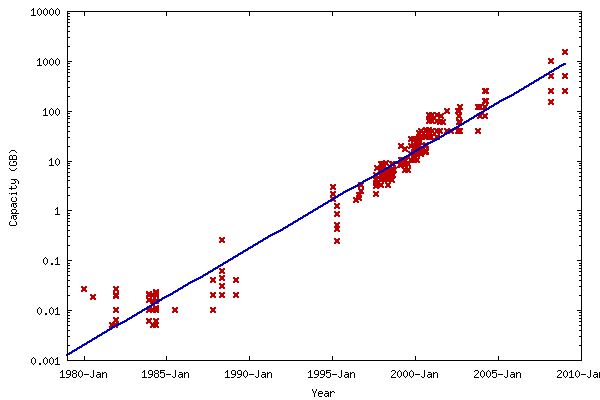
\includegraphics[width=\columnwidth]{figures/hardDriveCapacityOverTime.png}
\caption{A graph showing the increase in hard drive capacity from 1980
  to 2010.  It should be noted that the y-axis is shown in a
  logarithmic scale.  Image from Wikipedia.}
\label{fig:hardDriveCapacityOverTime}
\end{figure}

Many such archives that were previously stored on analog magnetic tape
have begun to be digitized, analyzed and presented to the research
community and public through online web resources.  The Cornell Lab of
Ornithology is one such organization and has recently made available a
huge amount of the recordings of birds through their
website \footnote{\url{http://macaulaylibrary.org/}}, the Macaulay
Library \cite{macaulay2007library}, and contains more than 175,000
audio recordings.  Another project from the Alberta Biodiversity
Monitoring Institute to monitor the biodiversity of birds using teams
that manually record audio has been operating since 2002 and has
collected approximately 8,800 individual 10 minute recordings
\cite{boutin2009abmi}, with more each year as the project ramps up.
This year they collected approximately 1,800 new recordings and expect
to collect increasingly more each year.

Here at the University of Victoria, I have developed the Orchive, one
of the largest repositories of bioacoustic data in the world,
containing over \aboutNumberOfOrchiveRecordings hours of recordings of
orca vocalizations, collected from OrcaLab, a land-based research
station at Hanson Island on the BC coast.  The Orchive project is the
primary focus in this thesis and the project will be described in
detail in Chapter \ref{chap:architecture} and results from using the
system developed in this thesis to this dataset in Chapter
\ref{chap:evaluation}.

In recent years, the larger storage and computational capacity of
computers has inspired researchers to analyze larger and larger
collections of bioacoustic data.  Much of the historical audio
recordings are present on audio tapes, and using high-throughput audio
digitization facilities, this data has begun to be transferred to
digital form.  At the University of Victoria, we have previously
described a project called the Orchive \cite{ness2013orchive} where we
have digitized over \aboutNumberOfOrchiveRecordings hours recordings
from the OrcaLab research facility, stored originally on 45 minute
long analog audio cassette tapes.  These recordings contain large
numbers of the vocalizations of orcas (\textit{Orcinus orca}) along
with other species of marine mammals.

The same advances in computer storage technology have led to
researchers becoming even more adventurous in the collection of large
amounts of bioacoustic data, skipping the process of recording onto
analog tape and recording directly into the computer. The
VENUS \footnote{\url{http://venus.uvic.ca/}} and
NEPTUNE \footnote{\url{http://www.neptunecanada.com/}}projects are
cabled undersea observatories that continuously record many kinds of
data, including salinity, pressure and video, and of relevance to this
thesis, audio data.  Another such project to continuously record audio
data is from the Cornell Lab of Ornithology, and is a project to
remotely record the vocalizations of right whales in the Atlantic.  In
this project, researchers have deployed a set of 8 buoys recording
audio continuously from 2008 to the present, and have collected over
100,000 hours of audio from these remote sensors
\cite{urazghildiiev2009rightwhale}.  The Cornell Lab of Orthinology
has another program to record the vocalizations of blue whales in
the eastern Atlantic that has collected a comparable amount of data.
There are many such projects, and more and more of them are being
started over time.

The amount of audio data recorded by these various projects is truly
immense, and in order for researchers to make sense of this data,
tools to navigate, listen to, annotate, analyze and classify it are
becoming increasingly more important.  Cornell University has
developed such a system which allows for researchers to access a
central repository of data from their workstations using
MATLAB \footnote{\url{http://www.mathworks.com/products/matlab/}}, and
it is being used to find the vocalizations of right whales and to
monitor the behaviour and population of this threatened species.

This thesis describes work in applying advanced audio feature
extraction, analysis and visualization tools to the study of large
archives of bioacoustic data.  It focuses on the data from the Orchive
but can be used for other sources of bioacoustic data as well.  There
are three distinct types of tools that will be demonstrated.  The
first are tools to extract features and analyze audio.  The second set
of tools are web-based and allow users from around the world to
collaboratively view and analyze the results obtained from the first
set of tools and to iteratively use them in combination with machine
learning systems to classify audio.  The third set are interfaces that
use a casual game metaphor to allow citizen scientists to help provide
annotations on this audio.

An aspect characterizing this work is the need to collaborate with
domain experts in the vocalizations of the biological species of
interest, and a large amount of the effort in this project is devoted
to the development of web-based interfaces that allow domain experts
with varying degrees of computer sophistication to access, create
annotations for our machine learning systems, and make sense of the
extracted data that our tools produce.  Thus, the core part of this
work is to bring tools, data, biologists, computer scientists, and
citizen scientists together into a collaborative partnership.

Most of the recordings studied by biologists are of a single species
and are with high quality recording gear under controlled conditions.
In bioacoustic databases collected via Passive Acoustic Monitoring
(PAM), this is often not the case.  In the cases of large bioacoustic
databases, recordings are often taken from a single location or a
number of locations, and how close animals are to the recording
devices can change dramatically during a recording.  There are often
also many sources of other sound in the recording, from environmental
noise like wind, to human produced noise from boats or
cars. Also, in many cases there are a variety of different animals
making sound in a recording, and these sounds can overlap each other.
While some bioacoustic recordings are well segmented, such as those of
the recordings of bird songs from the Cornell Lab of Ornithology, in
many cases of continuous recordings, the locations of the bioacoustic
sounds are not localized in time, and these recordings must be
annotated and segmented before they can be analyzed.

In most studies of bioacoustics up to the present time, individual
researchers record the sounds of the animals that they are interested
in studying.  In the process of doing the recording, they make notes
and record other kinds of metadata about the audio they record.  The
amount of audio that is typically analyzed is in the range of hundreds
to a few thousand recordings.  Even in larger studies such as those by
Harald Yurk \cite{yurk2002cultural} on the vocalizations of orcas, the dataset is of the order
of 1000 recordings.  These recordings are typically analyzed on a
single computer using software such as Raven \cite{cornell2011raven}, a
powerful tool for the study of bioacoustic data produced by the
Cornell Lab of Ornithology.  This software allows researchers to
record, import, view, analyze and annotate recordings and provides
ways to export the annotations to other programs that can be used to
further analyze the audio.  It works best with shorter audio files,
although large files can be read in and viewed using a paging
metaphor where sections of several minutes of audio are visualized at
a time.

The large size of these datasets also present a challenge for
developers and users of audio feature extraction and machine learning
algorithms in the field of Music Information Retrieval (MIR).  These
algorithms are often computationally intensive and require the use of
large clusters of computers.  In addition, the raw data used for the
calculations must be stored in such a way that all processing
computers can access it.

It is also important for researchers to be able to collaborate on
these large scale projects, to share their annotations, audio data,
and the raw results of their analysis with colleagues.  In order to do
this, one possible approach would be to use a web-based system, where
the individual researcher can connect to a large server-based system
that presents the data to them in an easy to use form, allows them to
make and share annotations, and connects to large amounts of computing
resources for them to perform audio feature extraction, machine
learning and other forms of analysis on their data.
 
Web-based software has been helping connect communities of researchers
since its inception \cite{bernerslee1992www}.  Recently, advances in
software and in computer power have dramatically widened its possible
applications to include a wide variety of multimedia content.  These
advances have been primarily in the business community, and the tools
developed are just starting to be used by academics. In our lab, we
have been working on applying these technologies to ongoing
collaborative projects that I am involved in
\cite{ness2008chants}. By leveraging several new technologies
including HTML5/Javascript,
Node.js \footnote{\url{http://nodejs.org/}} and
Python \footnote{\url{http://www.python.org/}}, I have been able to
rapidly develop web-based tools.  Rapid prototyping and iterative
development have been key elements of our collaborative
strategy. Although the number of users interested in the analysis of
large bioacoustic recordings is limited compared to other areas of
multimedia analysis and retrieval, this is to some degree compensated
by their passion and willingness to work closely with us in developing
these tools.

This work draws on ideas and concepts from many disciplines.  Because
of this it is essential to include definitions of these concepts.
These are presented in the Glossary (Appendix \ref{chap:glossary}).

%
% OrcaLab and the Orchive
%
\section{OrcaLab and the Orchive}
\label{section:introduction:orchive}

The whale species \textit{Orcinus orca}, commonly known as Killer
Whales \cite{ford2000book}, are large toothed whales found around the
world, in places as far afield as Antarctica and Alaska
\cite{estes2009decline}.  Two photographs of orcas are shown in Figures
\ref{fig:orcasSwimming} and \ref{fig:orcaBaby}.

\begin{figure}[t]
\centering
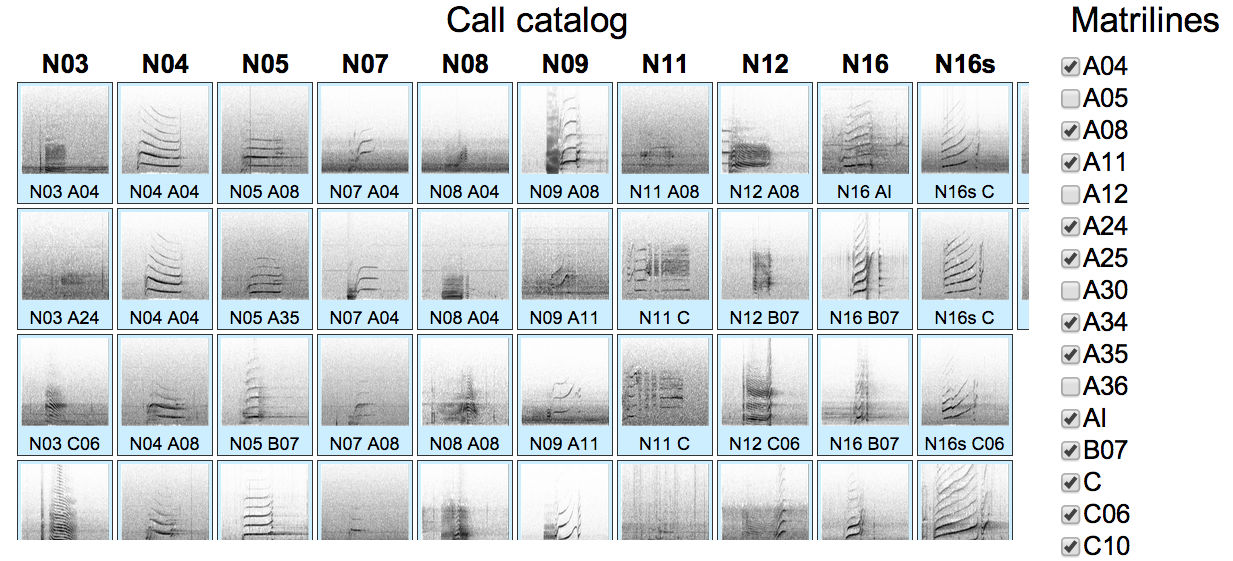
\includegraphics[width=\columnwidth]{figures/orcaCallCatalog}
\caption{An image showing spectrograms of a number of different orca
  call types from the NRKW.  The interface
  allows the researcher to display the call types from just a select number
  of pods and matrilines.}
\label{fig:orcaCallCatalog}
\end{figure}

\begin{figure}[t]
\centering
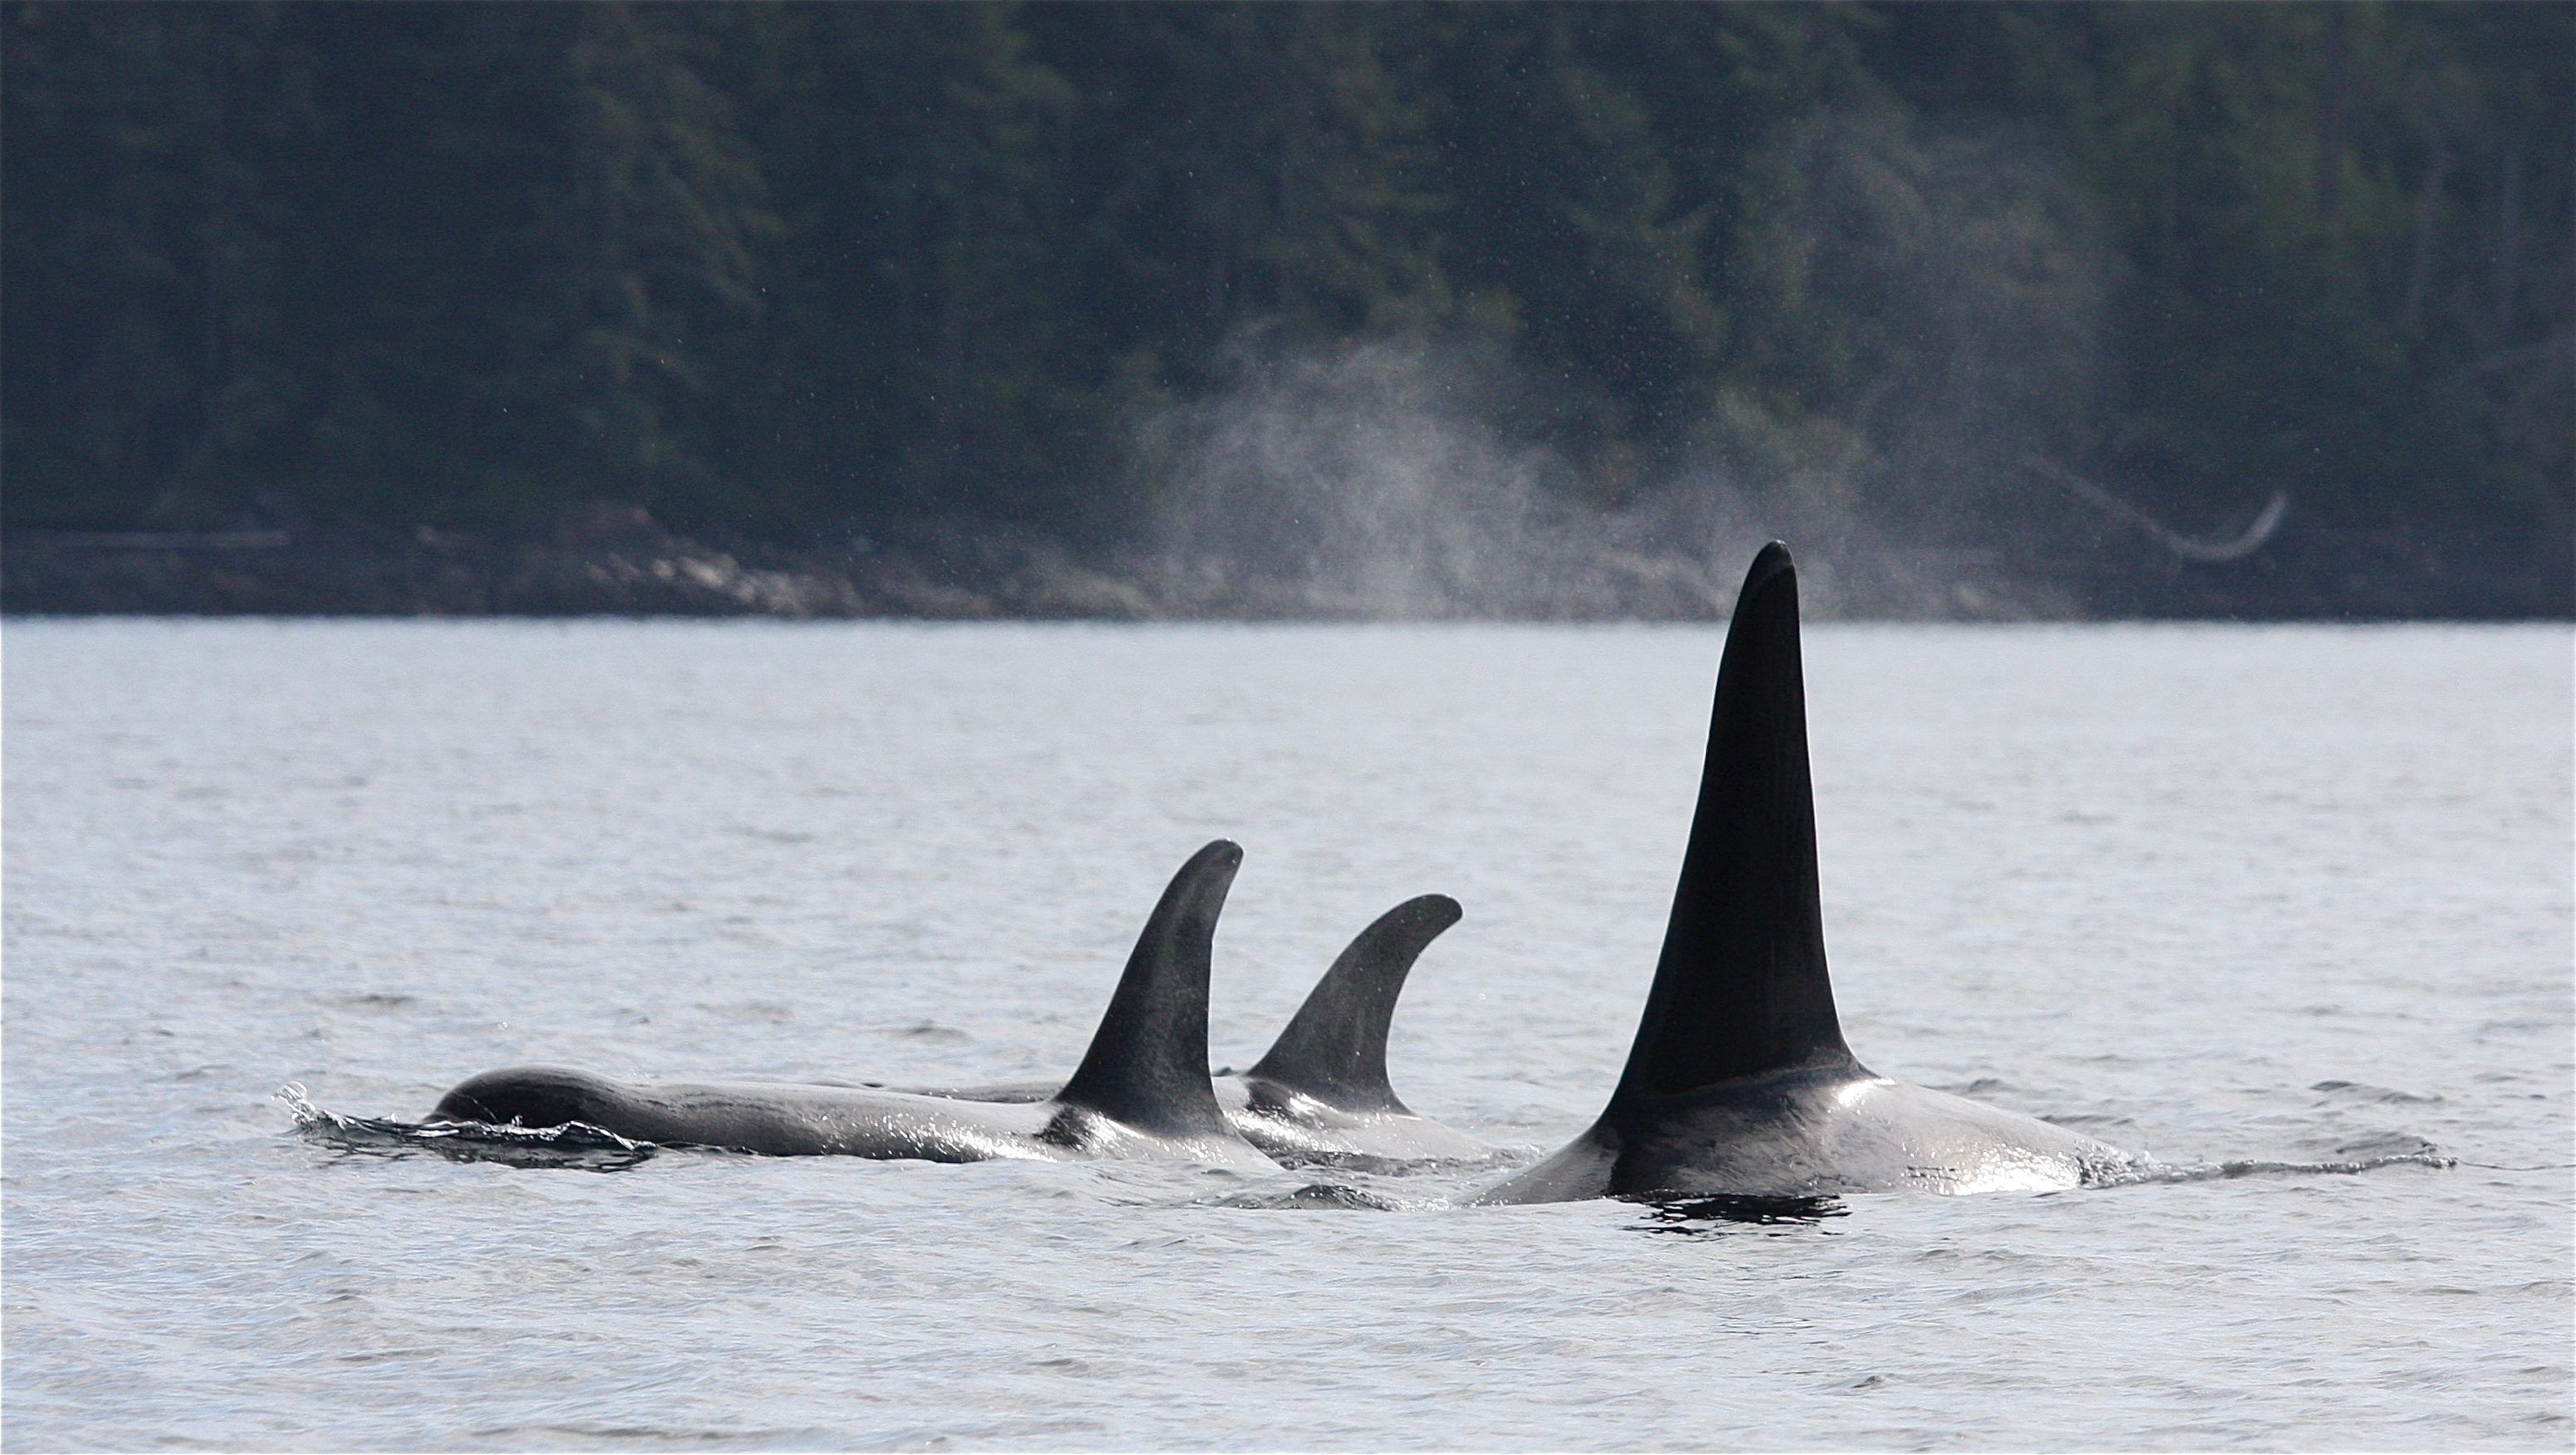
\includegraphics[width=\columnwidth]{figures/orcasSwimming}
\caption{A photograph of the A34 matriline of orcas swimming near
  OrcaLab.  The tall straight fin belongs to an adult male and the
  smaller, curved dorsal fins are indicative of female and juvenile
  orcas.  Photo credit OrcaLab.}
\label{fig:orcasSwimming}
\end{figure}

Orcas make three types of vocalizations, echolocation clicks, whistles
and pulsed calls.  The pulsed calls are stereotyped vocalizations,
which have been classified into a catalog of over 52 different call
types by John Ford \cite{ford1987catalogue}.  Of the 18,000
annotations currently in the Orchive, 3000 are individually classified
call types.  In addition, OrcaLab has created a call catalog
containing 384 different recordings of different call types vocalized
by a variety of different pods and matrilines.  A picture showing
spectrograms of a variety of different call types is shown in Figure
\ref{fig:orcaCallCatalog}.


\begin{figure}[t]
\centering
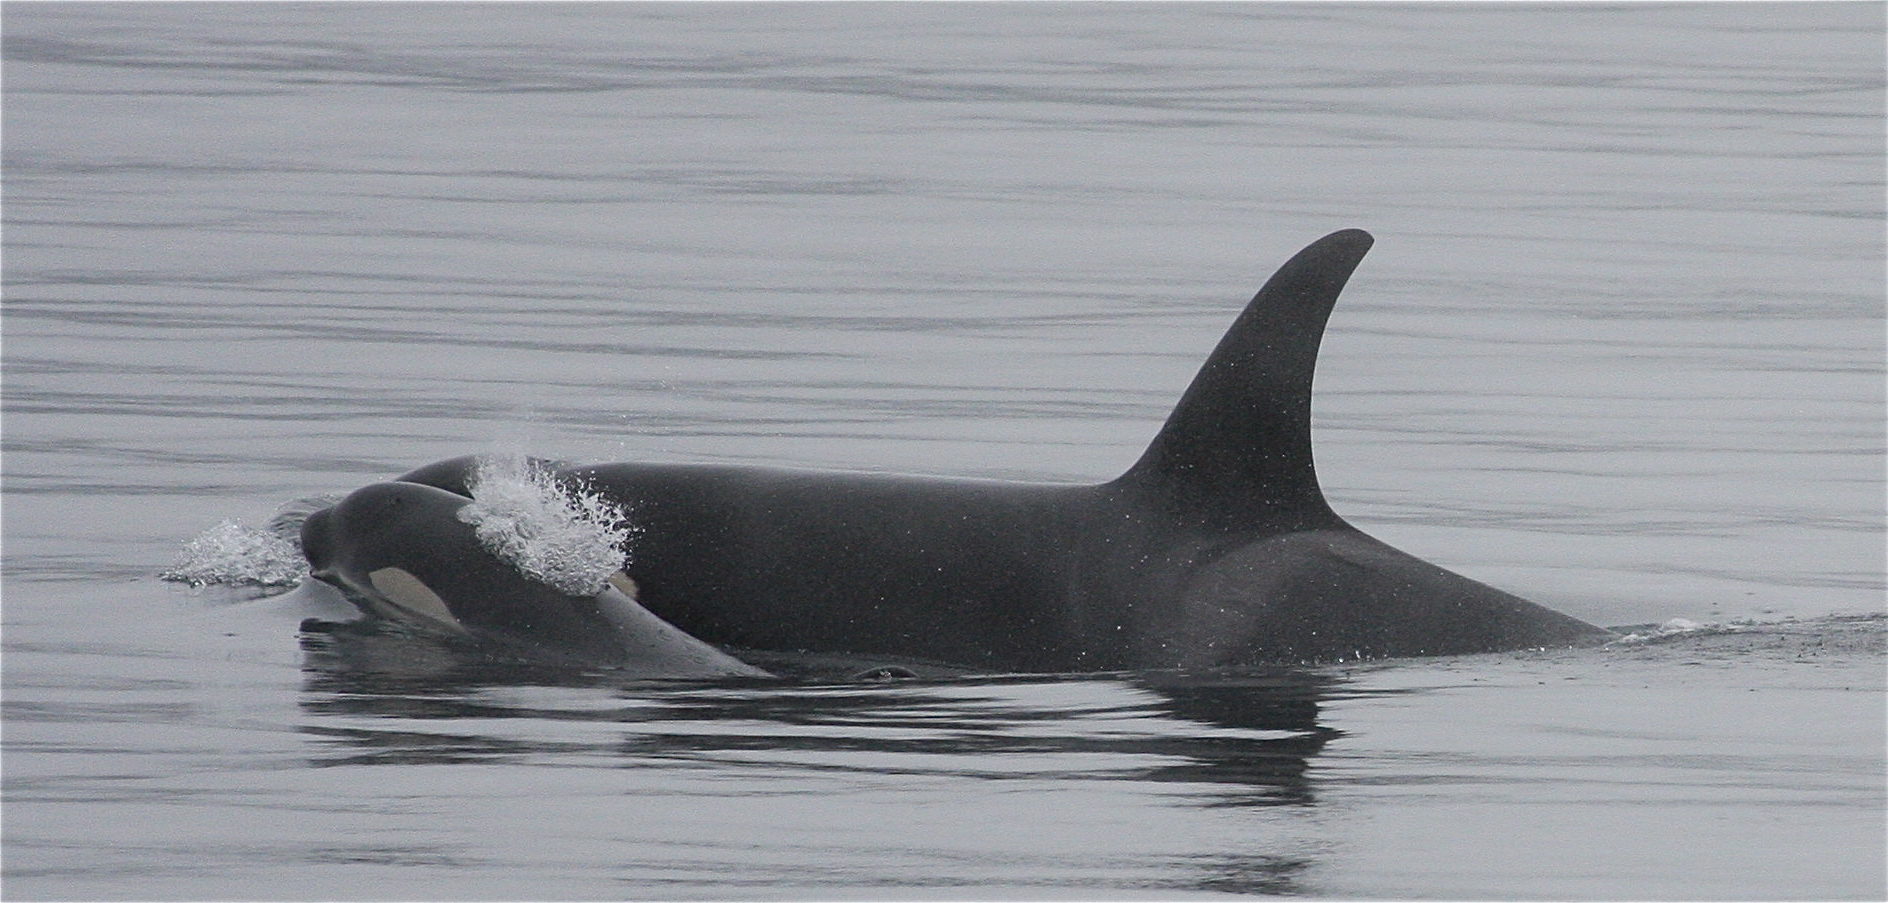
\includegraphics[width=\columnwidth]{figures/orcaBaby}
\caption{A photograph of an orca and her calf A42. Photo credit OrcaLab.}
\label{fig:orcaBaby}
\end{figure}

In 1970 Dr. Paul Spong, an orca researcher, founded OrcaLab on Hanson
Island, an area frequented by different pods of the northern resident
killer whale (NRKW) community due to the concentration of salmon in
this area.  He founded OrcaLab after having experiences with two
whales in the Vancouver Aquarium, ``Skana'' and ``Hyak'' that showed
their capability to communicate. Figure \ref{fig:orcalabMap} shows a
map of the area near Hanson Island.

\begin{figure}[t]
\centering
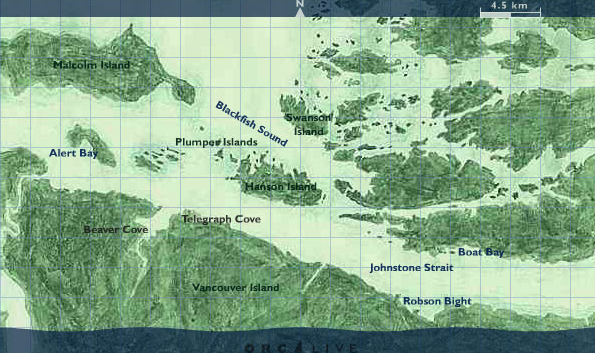
\includegraphics[width=\columnwidth]{figures/orcalabMap}
\caption{A map showing the location of OrcaLab, on Hanson Island and
  the arrangement of the other islands where hydrophones were placed.
  The Robson Bight Michael Bigg Ecological Reserve is shown near the
  bottom of the map and represents a prime habitat for salmon and
  orcas.}
\label{fig:orcalabMap}
\end{figure}

Over the years, the research camp developed into a permanent 24/7,
land-based research station with a network of hydrophones off the
nearby islands, giving OrcaLab a wide acoustic horizon, able to hear
whales coming in north from the Johnstone Strait and heading toward
the Michael Biggs (Robson Bight) Ecological Reserve.  It was hoped
that by having hydrophones anchored to land, the orcas would be less
disturbed, and it would be considerably less costly, than if they were
followed in a specialized boat.  A photograph of the OrcaLab research
station is show in Figure \ref{fig:orcaLab}, on the south facing side
a large number of solar panels is visible.  OrcaLab is completely off
the grid, and maintaining it is a considerable task, and involves
dealing with harsh weather, generators, stacks of deep cycle marine
batteries.

During the winter there are very few sightings of orcas around Hanson
Island and only one or two people stay out there at a time.  During
the summer though, the lab becomes very active as around a dozen young
research assistants come to help listen to and record the
vocalizations of orcas.  A photograph showing a number of these
researchers on the deck of the main OrcaLab research lab watching for
whales with binoculars is in Figure \ref{fig:orcaLabOnDeck}.  An
inside view of the lab is shown in Figure \ref{fig:orcaLabWork} where
two research assistants are listening to the hydrophones on
headphones, writing notes in a lab book, and adjusting levels on an
audio mixer.  When the tapes have been recorded, they are stored
upstairs in the lab in stacks on shelves, as can be seen in Figure
\ref{fig:orcaTapes}.

\begin{figure}[t]
\centering
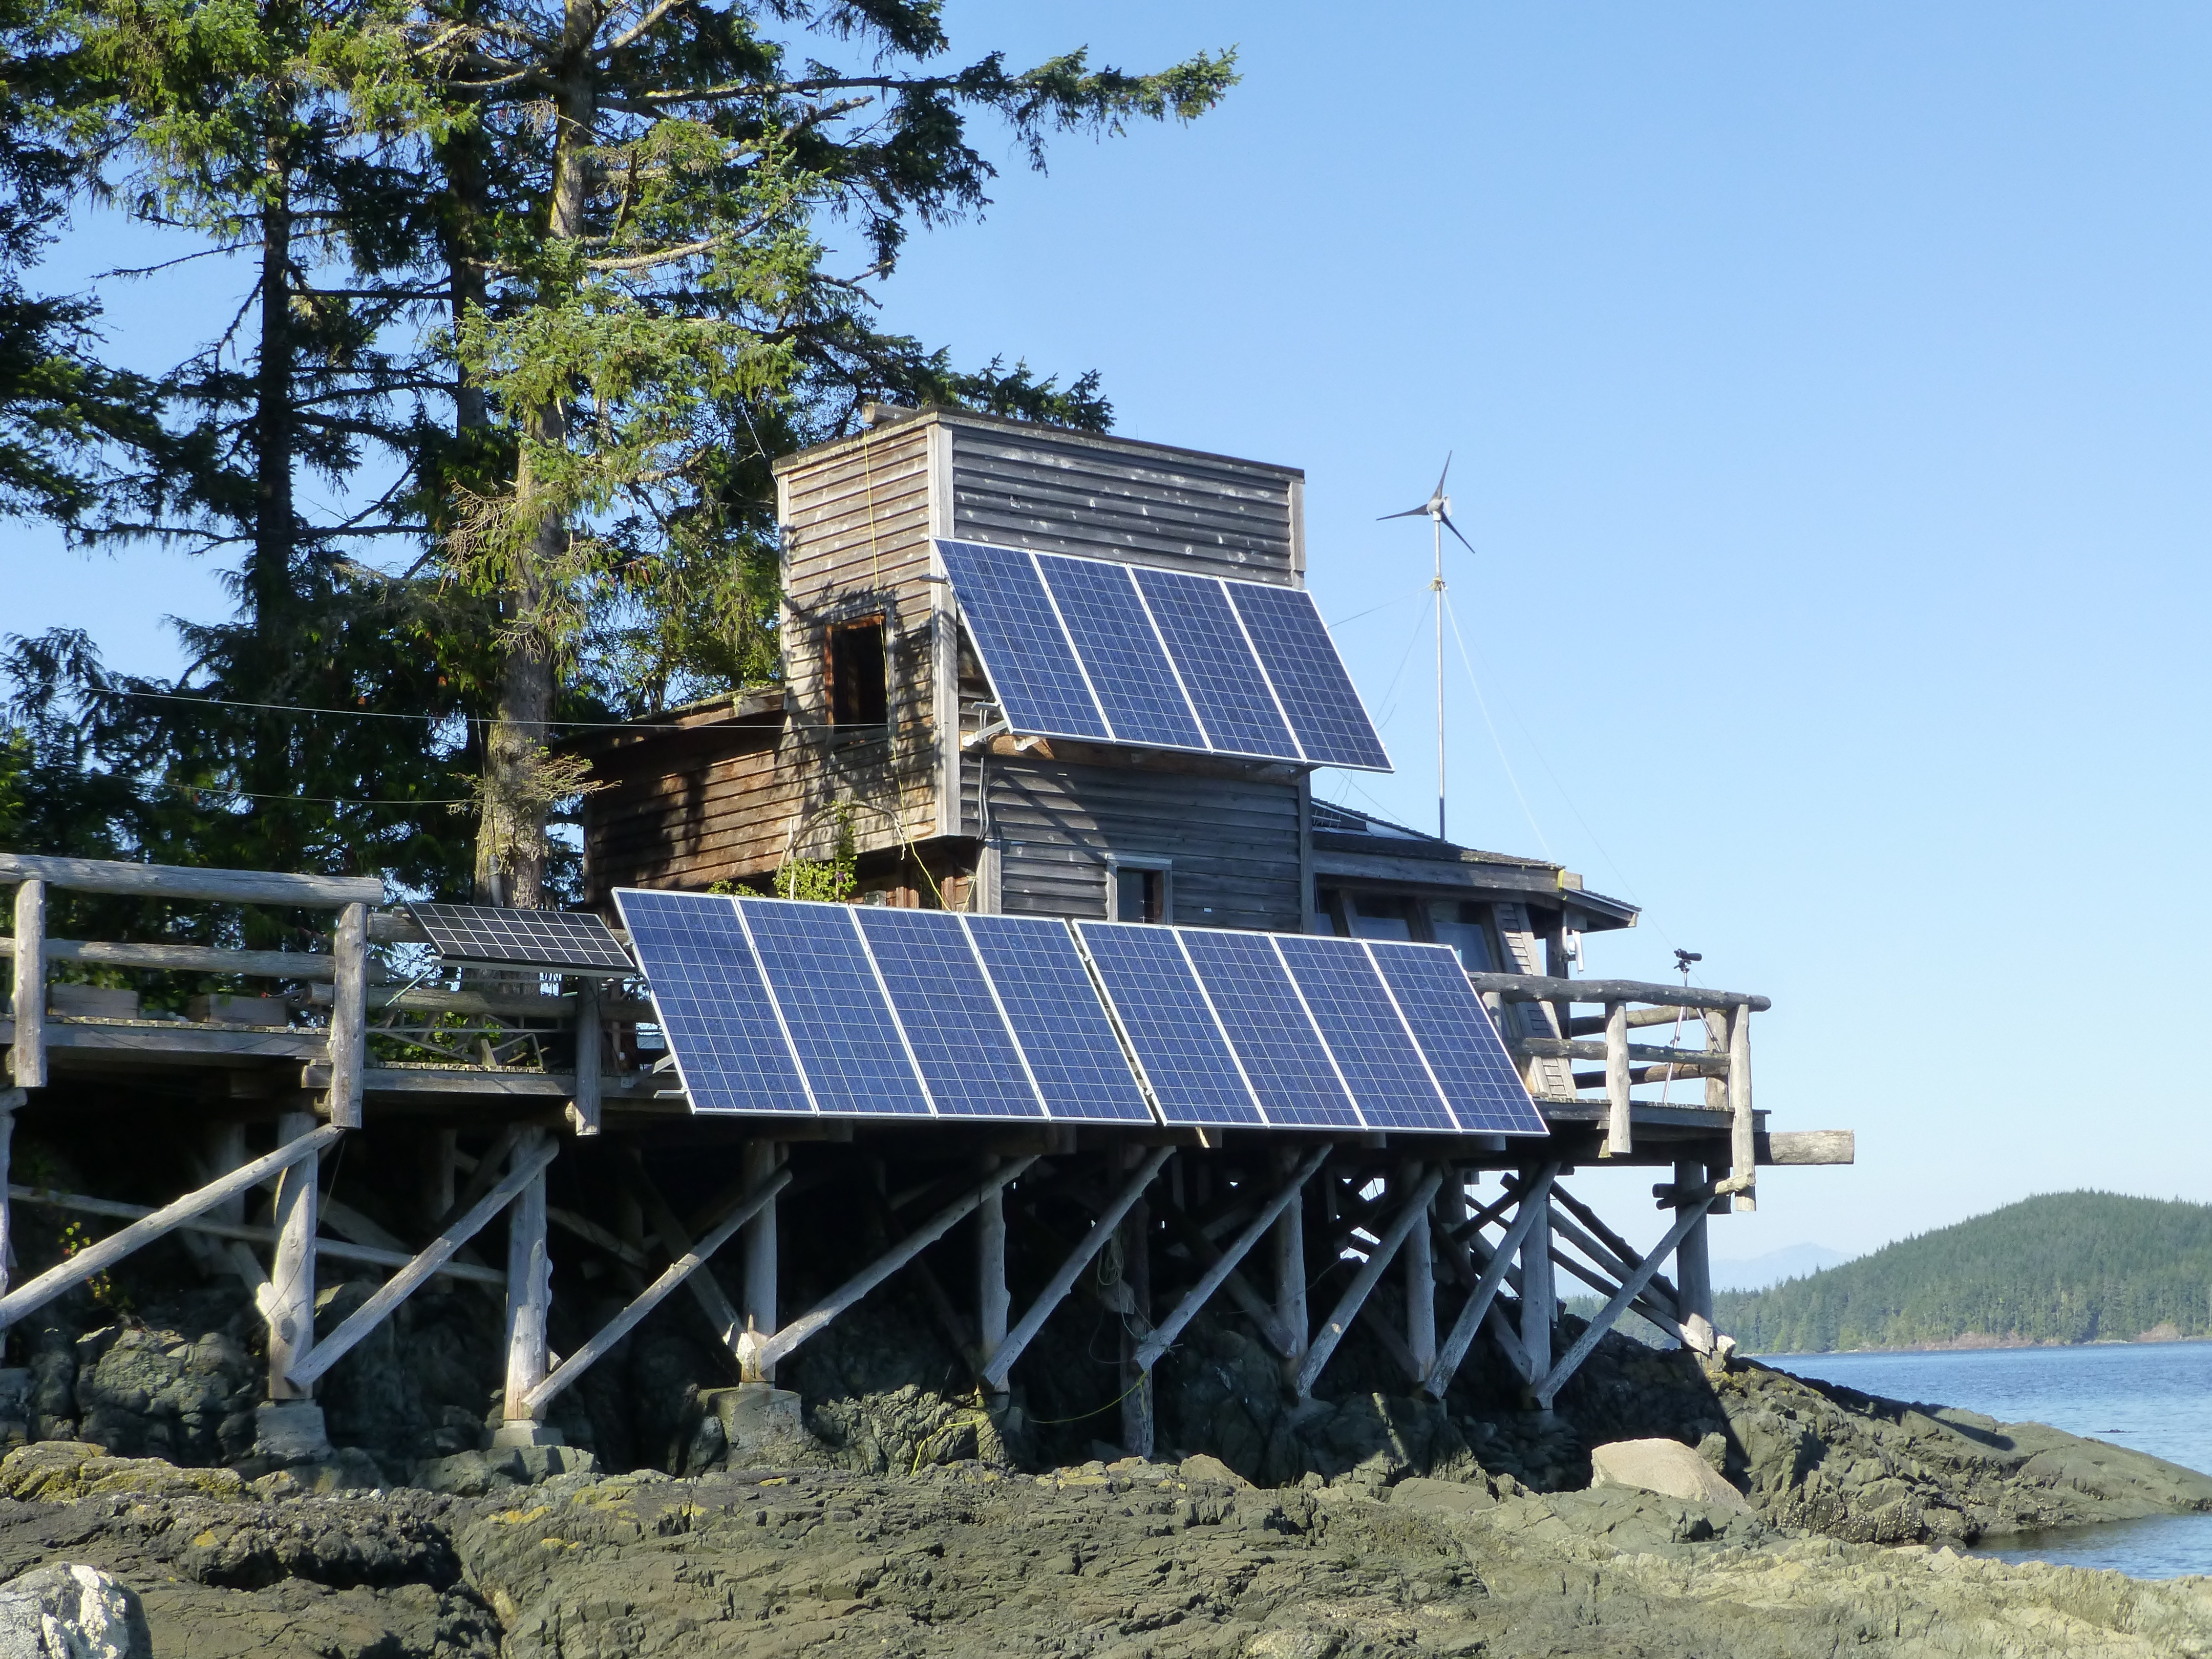
\includegraphics[width=\columnwidth]{figures/orcaLab}
\caption{A photograph showing OrcaLab on Hanson Island.  In the
  foreground on stilts is the land-based research station, with three
  sets of solar panels covering its southern face.  A deck where
  visual observations can be made surrounds the ground level of the
  lab.  At the top of the lab is where most of the audio cassettes are
  stored and where research on the recordings of OrcaLab is ongoing
  using a combination of analog and digital technology. Photo credit OrcaLab.}
\label{fig:orcaLab}
\end{figure}

\begin{figure}[t]
\centering
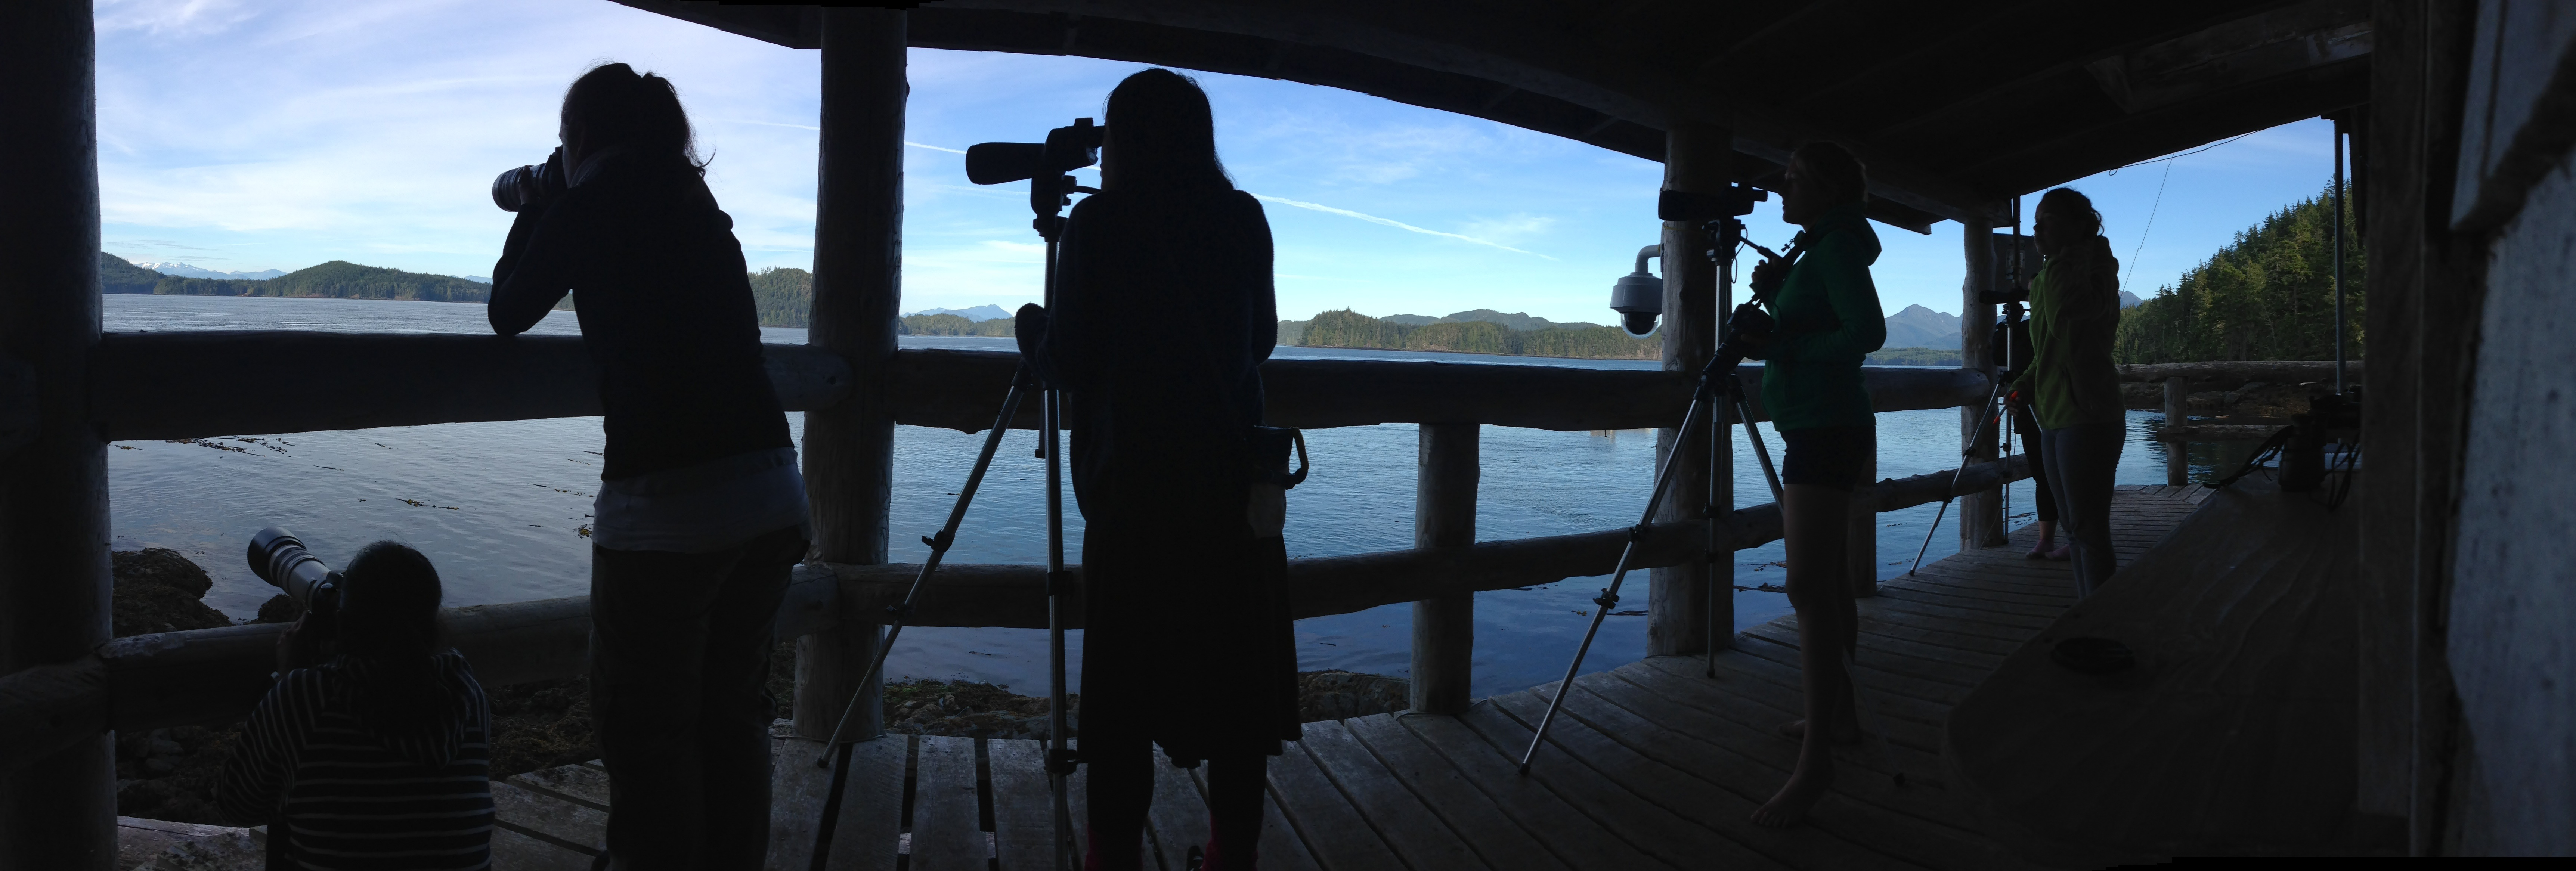
\includegraphics[width=\columnwidth]{figures/orcaLabOnDeck}
\caption{A photo of a group of summer research assistants making photo
  identifications of whales on the deck of the main OrcaLab research
  facility.  Photo credit OrcaLab.}
\label{fig:orcaLabOnDeck}
\end{figure}

\begin{figure}[t]
\centering
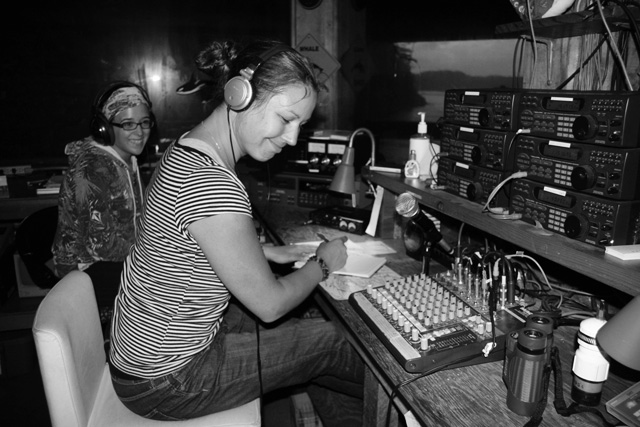
\includegraphics[width=\columnwidth]{figures/orcaLabWork}
\caption{A photograph showing the inside of the OrcaLab research
  station, with a research assistant taking notes in a lab book
  as she listens to hydrophones and adjust a multi-track mixer.  Other
  equipment that can be seen are VHF radios, binoculars, audio and
  Digital Audio Tape (DAT) tape recorders and a microphone for making
  voice notes.  On the front wall is a little sign that has arrows for
  North and South to help orient new summer research assistants. Photo
  credit OrcaLab.}
\label{fig:orcaLabWork}
\end{figure}

\begin{figure}[t]
\centering
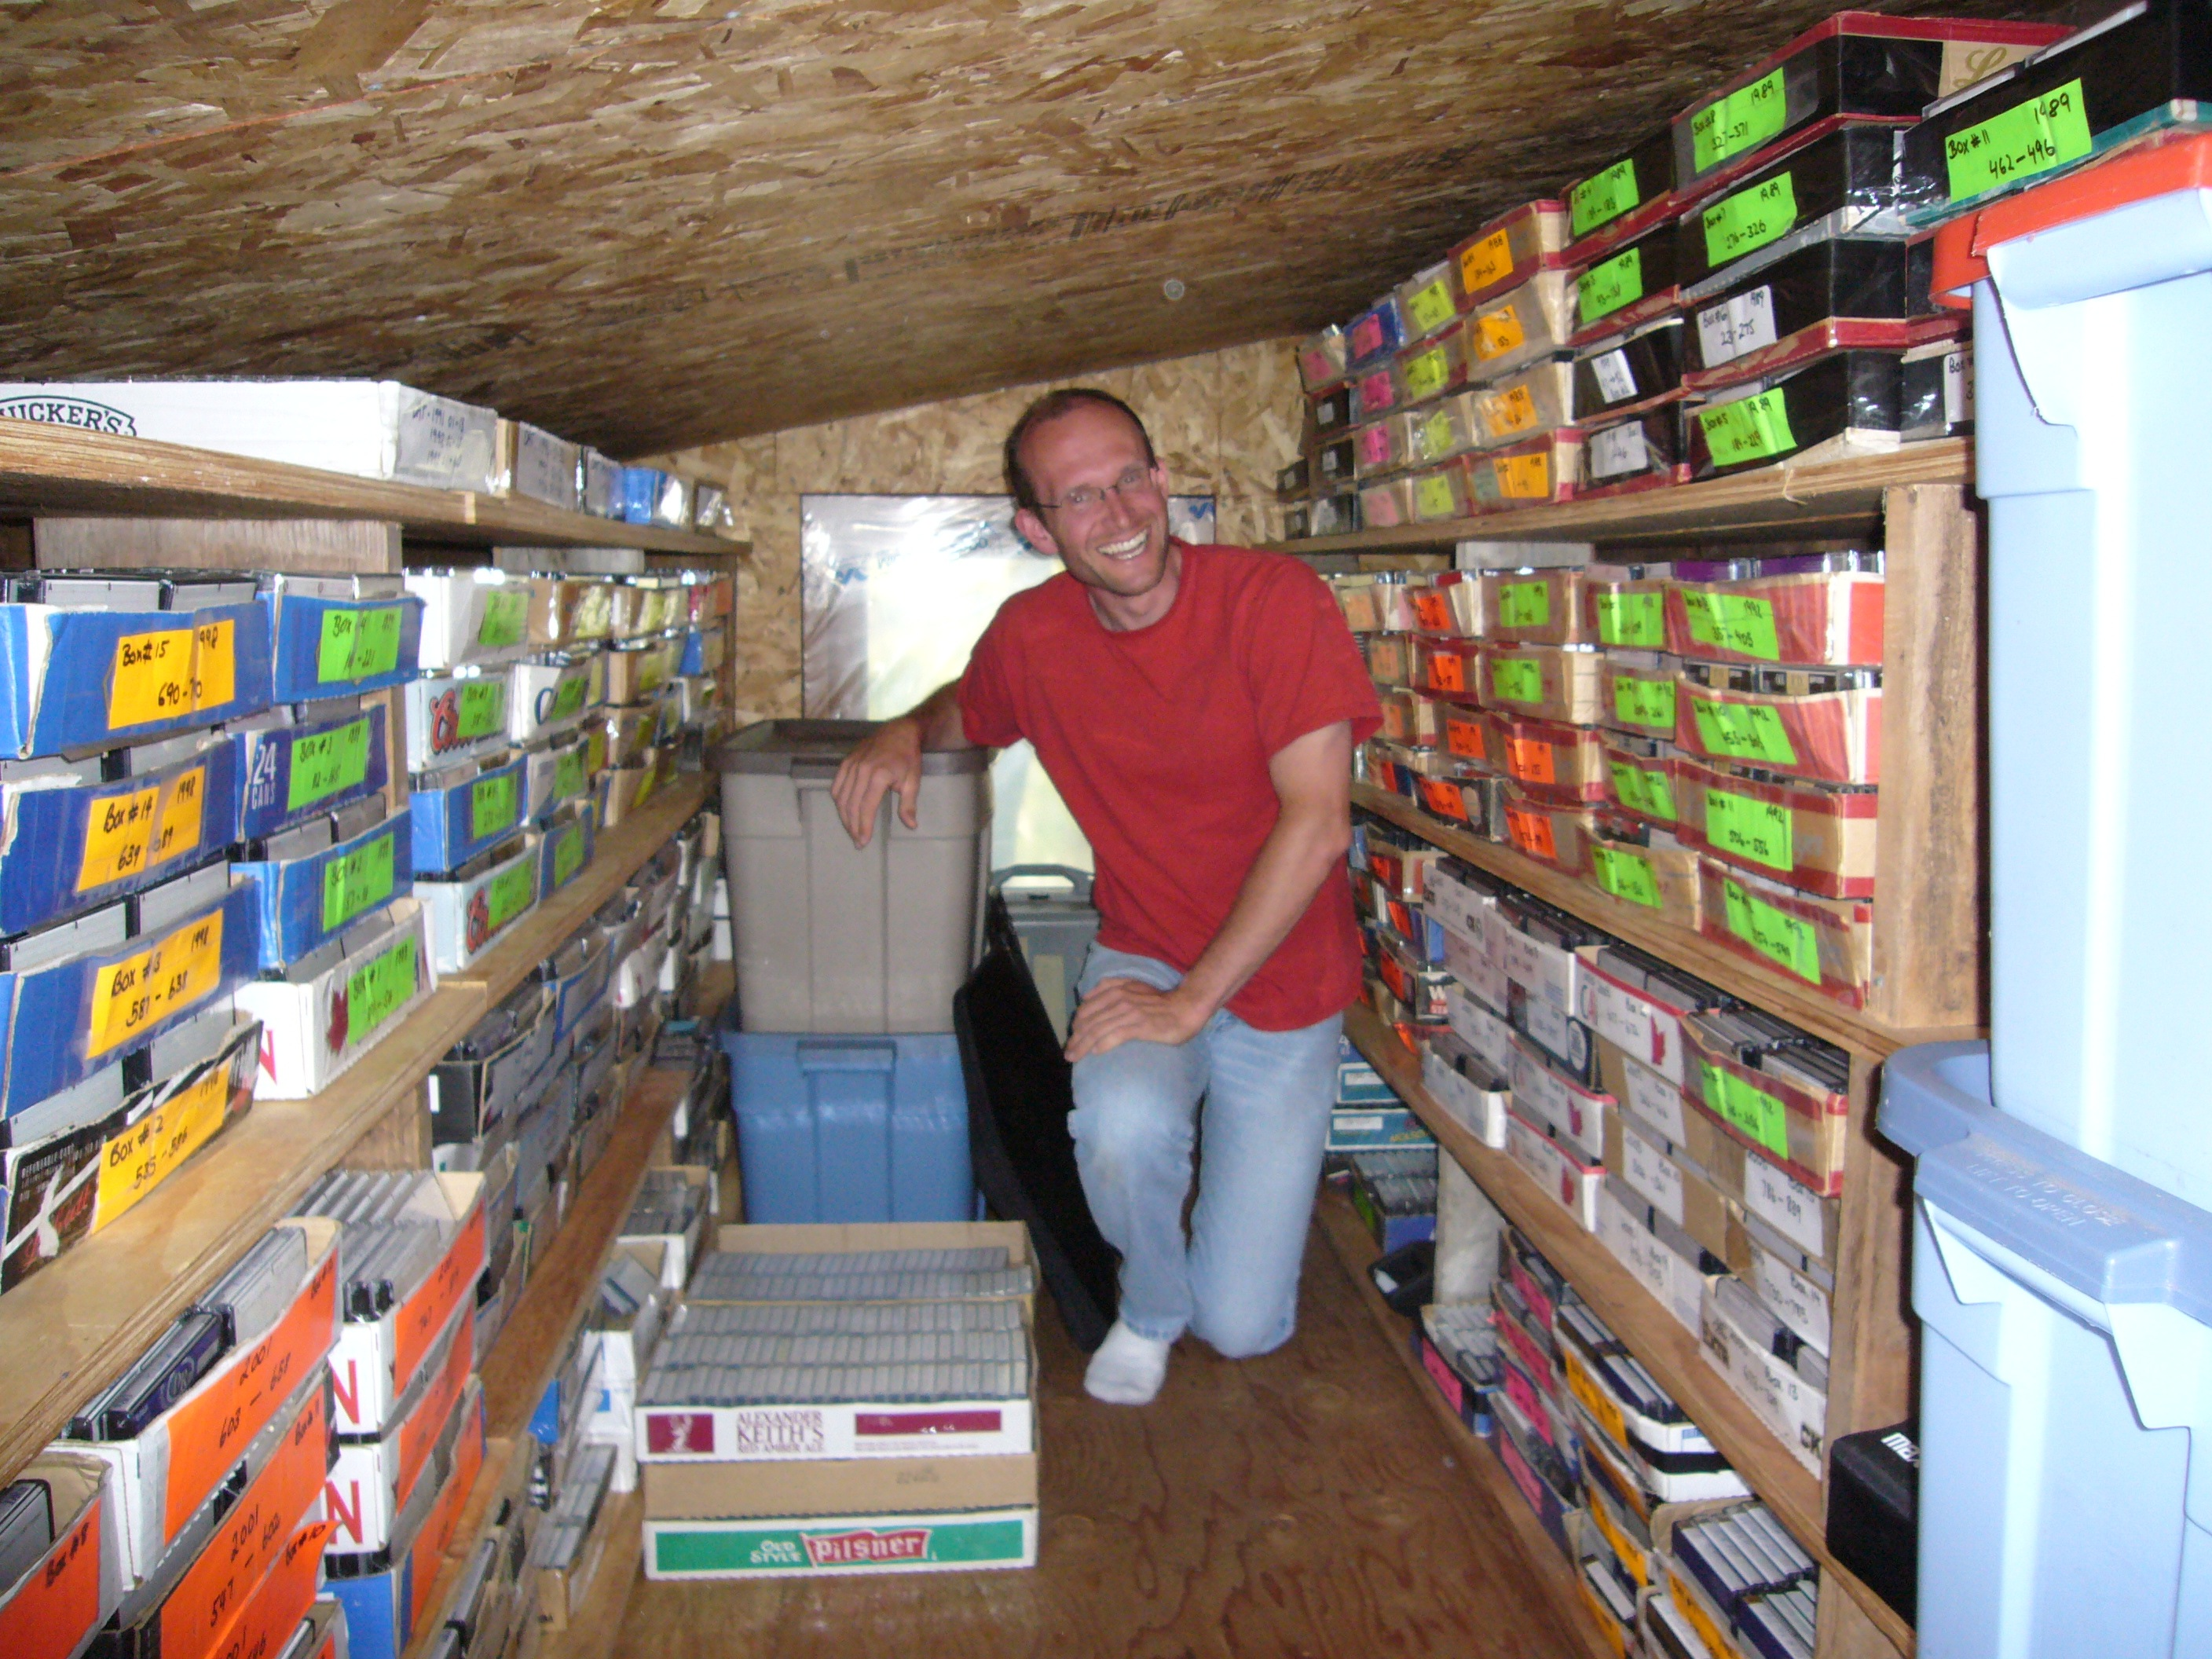
\includegraphics[width=\columnwidth]{figures/orcaTapes}
\caption{A snapshot of the author with some of the many analog
  cassette tapes that are in storage above the main lab at
  OrcaLab. Photo credit OrcaLab.}
\label{fig:orcaTapes}
\end{figure}


\begin{figure}[t]
\centering
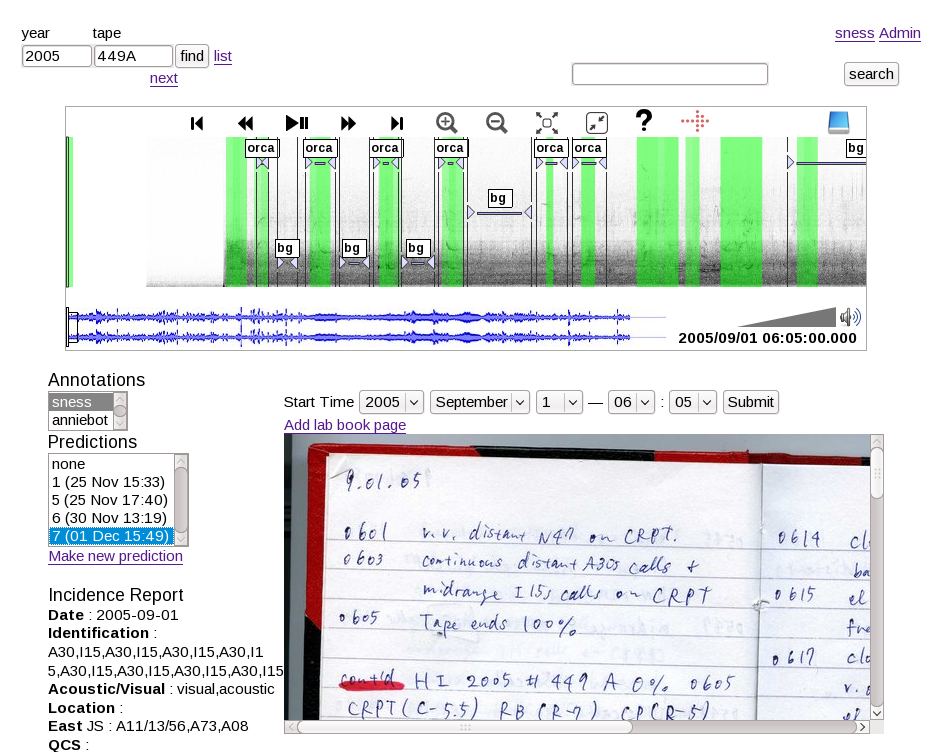
\includegraphics[width=\columnwidth]{figures/orchiveFull}
\caption{The researchers at OrcaLab have collected many overlapping
  and complementary sets of data.  Besides audio recordings, detailed
  lab books with timed comments that describe the tape and the
  conditions, along with considerable other information and derived
  knowledge.  Other information that is collected is a daily incidence
  report telling which orcas are in the area.  All of this data can be
  visualized in the Orchive interface as seen above.}
\label{fig:orchiveFull}
\end{figure}

A huge amount of data is collected at OrcaLab in addition to the
recordings.  The largest and richest of these is a set of lab books
that have been kept since 1983 and give details about the location,
behaviour and identity of the orcas.  The lines in the lab book page
are given minute numbers, and often one 45 minute recording will
stretch over two to three pages.  In addition to this information,
photos and videos are captured and archived, incidence reports about
which whales are in the area for a 10 year time span, hand drawn maps
of orca routes on specific days are amongst the many and varied forms
of data they have.  A small segment of this is shown in the Orchive
V1.0 interface show in Figure \ref{fig:orchiveFull}.

The goal of the Orchive project is to digitize acoustic data that have
been collected over a period of \totalYearsOrcaLabCollecting years
using a variety of analog and digital media at the research station
OrcaLab \footnote{\url{http://www.orcalab.org}} on Hanson Island on
the west coast of Vancouver Island in Canada.  Currently, they have
approximately \aboutHoursOfOrchiveRecordings hours of analog
recordings, mostly in high quality audio cassettes. In addition to the
digitization effort which after 7 years of work was recently
completed, our research lab is developing algorithms and software
tools to facilitate access and retrieval for this large audio
collection.  The size of this collection makes access and retrieval
especially challenging (for example, it would take approximately 2.2
years of continuous listening to cover the entire archive).
Therefore, the developed algorithms and tools are essential for
effective long-term studies employing acoustic techniques. Currently,
such studies require enormous effort as the relevant acoustic tapes
need to be recovered and the relevant segments need to be tediously
digitized for analysis.

This archive of data is now available in electronic form which makes
it easier to access than when it was on a single set of analog tapes
at OrcaLab, what would make it even more useful to scientists would be
the ability to collaborate together on the process of annotating
audio, running experiments and analyzing results.

Although these recordings contain large amounts of Orca vocalizations,
the recordings also contain other sources of audio, including
voice-overs describing the current observing conditions, boat and
cruise-ship noise, and large sections of silence.  Finding the Orca
vocalizations on these tapes is a labor-intensive and time-consuming
task.

Many parts of the recordings contain boat noise, which makes
identifying orca call types both difficult and tiring. In addition,
the size of the Orchive makes full human annotation practically
impossible. Therefore, I have explored machine learning approaches to
the task.  One data mining task is to segment and label the recordings
with the labels background, orca, voice. Another is to subsequently
classify the pulsed orca calls into the call types specified in the
call catalog \cite{ford1987catalogue}.  Experiments involving these
two classification tasks will be explored in the Chapter
\ref{chap:evaluation} of this thesis.

There have been many goals of the OrcaLab project, and when asked,
Dr. Paul Spong provided the following quote:

\begin{quote}
`` OrcaLab was founded in 1970 as a field research campsite on Hanson
  Island, with the aim of observing orcas in the wild. The initiative
  followed Paul Spong's experiences with orcas in captivity at the
  Vancouver Aquarium, which convinced him that capture and confinement
  of orcas was unfair. The first summer season provided numerous
  insights, e.g. individuals could be identified and were observed
  repeatedly. OrcaLab's first hydrophone recordings were made that
  year. During the following decades, OrcaLab developed into a
  permanent research facility that monitors the surrounding underwater
  acoustic environment year round via a network of remote hydrophones.

  In the early 1970s, virtually nothing was known about orcas. The
  motivation for establishing OrcaLab was curiosity about orcas and
  their lives, along with concerns about the impacts of captivity on
  individual orcas and their populations. Though more difficult, it
  was felt that studies of orcas in the wild rather than in captivity
  would potentially yield more information about them.

  One of the most frequently asked questions about the calls orcas use
  is, what do they represent, and do they amount to language orcas use
  for meaningful communication? These are very difficult questions to
  answer.  In the meantime, the work of OrcaLab continues to refine
  call usage in order to improve tracking of orca movements,
  behaviours and associations within the Johnstone Strait Blackney
  Pass and Blackfish Sound area as covered by the hydrophone network.
  This 24/7 effort has enabled a fairly accurate picture of which
  orcas frequent this area and with whom they are traveling.  In
  turn, this long-term record has helped establish the area as Core
  Habitat in recognition of its importance to orcas.  The enduring
  nature of the 30 plus years of OrcaLab recordings, now preserved in
  the Orchive, will mean that in the future interesting questions
  about language may ultimately be addressed.  ``
\end{quote}

The research objectives of OrcaLab include studying the vocalizations
of orcas, of examining the effects of boat noise on orcas, the study
of the family structure of orca populations, the behaviour of orcas
and long term population studies on orcas.  


%
% MIR and Bioacoustics
%
\section{MIR and Bioacoustics}
\label{section:introduction:MIRandBioacoustics}

It has only been in recent years that computer hard drives and RAM
have become able to store the large amounts of data that is required
to represent sound.  This represents another big challenge and
opportunity at the same time for the field of bioacoustics, as it
allows for large amounts of audio data to be quickly accessible, and
for this data to be indexed and stored in databases and analyzed by
computers.  The field of Music Information Retrieval experienced a
similar blossoming in the early 2000's, when computer storage and
computational power became great enough to store and analyze the data
of songs.  The field of bioacoustics is just starting to show similar
growth, and the use of tools from the field of Music Information
Retrieval (MIR) on bioacoustic data has shown great promise.

There are many audio features that have been used in MIR, the simplest
are waveform features that look at the properties of the raw audio
signal.  Spectral Features use a Fast Fourier Transform (FFT) to break
a window of sound down into its characteristic frequencies, and many
statistical properties of these spectral have been explored as audio
features.  MFCCs were first developed in research into human speech,
have shown great promise in the field of MIR for a variety of tasks.
Chroma is an audio feature that wraps the entire spectrum into a 12
semitone musical scale, and is very useful when looking at music that
has notes or chords in it.

From these audio features, researchers in MIR use a variety of the
most advanced techniques in machine learning including Support Vector
Machines, Decision Trees, Non-Negative Matrix Factorization and Deep
Belief Networks.

There are a wide variety of academic and commercial applications of
MIR software, including playlist generation, tagging of songs
\cite{ness2009improving}, new music interfaces for musicians
\cite{ness2011gesture} and for listeners \cite{ness2009audioscapes}
and music recommendation \cite{miller2010geoshuffle} as is done in
Google Music\footnote{\url{http://music.google.com}},
Spotify\footnote{\url{https://www.spotify.com}} and
iTunes\footnote{\url{http://apple.com}}.

However, many of the tools developed for MIR are not well adapted for
the study of bioacoustic data.  When studying recorded songs, there is
often a large amount of well-curated meta-data for each song, For
example, when classifying songs based on genre, the artist, song
title, genre, record label and many other forms of data are available,
and boundaries between songs are clearly marked, and are often in
individual files.  Music often comes pre-segmented into songs, which
often have identifiable sections including verse and chorus, as well
as lower level features such as beat and tatum that facilitate
analysis by computers.  In addition, most work in MIR has been on
songs that were professionally recorded in a studio environment.

\subsection{Marsyas}
\label{sec:introduction:marsyas}

\textit{Marsyas} \cite{tzanetakis00} is a system used extensively in this
thesis to generate audio features and can also classify the features
using machine learning algorithms such as Support Vector Machines
(SVM) and Approximate Nearest Neighbours (ANN).  It uses a dataflow
architecture, similar to many other programs such as
MaxMSP\cite{puckette1998real} in which users connect objects that
process audio data by physically drawing lines between them on the
screen.  \textit{Marsyas} on the other hand uses an implicit patching metaphor
\cite{bray2005implicit} in which objects are nested within other
objects, and the flow of data is determined by the hierarchical
structure of \textit{Marsyas} subsystems (MarSystems).  This allows for faster
programming and development of new networks of audio feature
extractors and processors custom made for a specific audio problem.

\textit{Marsyas} forms part of the central core of the Orchive system as its
main audio feature extraction framework.

In orchive v1.0, in order to generate the precalculated spectrograms, a
program was added to \textit{Marsyas} to generate and save images of
spectrograms.  There also existed functionality in the web interface
to run audio feature extraction and machine learning jobs using
\textit{Marsyas} and to view the results overlayed on the spectrogram.  \textit{Marsyas}
was also extensively used in the creation of the website and
interfaces, like the call catalog.

In orchive v2.0, the Python bindings of \textit{Marsyas} have allowed us to
embed \textit{Marsyas} directly in the webserver and to deliver audio
features or spectrogram images on the fly.

In the course of work done for this thesis, this author added new
audio feature extraction subsystems to \textit{Marsyas}, including the porting
of the Yin pitch detector from Aubio \cite{brossier2006aubio} to
\textit{Marsyas}.  Aubio is a widely used audio feature extraction framework
that has a particularly efficient implementation of the YIN algorithm.
The first version of the Orchive was developed for my Masters thesis,
and the second version of the Orchive was developed for the work
described in this thesis.

Other work was carried out porting code from AIMC \cite{waltersphd} a
framework incorporating DSP models of the cochlea and peripheral
auditory system.  Work was done to port a variety of cochlear
models\cite{lyon2011hearing}\cite{lyon2011cas}, strobe finding and the
calculation of Stabilized Auditory Images \cite{patterson1992complex}.
In other work \cite{rehn2009sparse} these cochlear models have shown
to outperform \cite{chechik08} spectral methods
\cite{duda1990correlograms} and show the importance of the temporal
domain \cite{slaney1993time} when studying sounds made using a pulse
resonance model \cite{waltersphd} as are the vocalizations of orcas.


%
% Relevance of this work
%
\clearpage
\section{Relevance of this work}

An important aspect in the design of a tool to support collaborative
work is to consider what user communities will use the tool.  In the
case of the Orchive, there are a number of different scientific
communities that will be using this tool and the data this tool
provides access to.  

The primary scientific community that will benefit from this work will
be researchers interested in bioacoustics, machine learning, and music
information retrieval.  These scientists are typically computer
scientists with interests in Music Information Retrieval and
bioacoustics.  This archive represents a site where researchers can
get large amounts of high quality and uniformly collected data.
Researchers interested in bioacoustic algorithms have different goals
and skill sets from cetacean biologists, for example, many have
extensive knowledge of Digital Signal Processing and audio feature
extraction algorithms.  This system should be flexible and powerful
enough to allow these researchers to ask questions that are relevant
to them.  The required features for this group of users include
allowing them to choose different audio feature extraction algorithms
and to then take the resulting data and run it against a variety of
machine learning algorithms in as flexible a manner as possible.  It
should allow them to quickly obtain annotations from audio, where the
annotations can be from experts in the species being studies, citizen
scientists and the output of machine learning algorithm.  They then
often want to obtain either the raw audio of those annotated regions
in the case of scientists with more of a MIR background or audio
features as is the case with specialists in machine learning.  They
then optionally would often like to view the results of their audio
feature extraction and machine learning algorithms directly to be able
to listen to the sound and see the output of their algorithm in the
same interface, as is often done with Sonic Visualiser
\cite{cannam2010sonic} or Raven \cite{ravenpro}.  The system described
in this thesis has functionality to perform all of these tasks as will
be demonstrated in later chapters.

Another community that might gain benefit from the Orchive are
researchers interested in studying the NRKW.  Before the creation of the Orchive, if a biologist was
interested in studying the vocalizations of the NRKW as recorded by
OrcaLab, they would first have to drive 7 hours up Vancouver Island
from Victoria, and then contact Dr. Spong and arrange for him to pick
them up on a boat, or perhas kayak across the Johnstone Strait as was
done by some researchers \cite{deecke1999quantifying}. They would then
have to look through lab books and find the cassette tape they were
interested in studying.  This cassette would then be used to study the
vocalizations by listening and fast forwarding and rewinding.  The
researcher would then make annotations in their own lab books and
would record the data they were interested in studying.  Each
researcher traditionally then keeps the annotations and data generated
from this procedure themselves.  If future researchers want to obtain
this data for further analysis, they must first be aware of the fact
that this researcher has the data and then request it from them.  With
the distributed collaborative system I have designed, not only can
these biologists easily listen to any recording in the entire archive
from any internet connected computer in the world, and compare
different recordings, they can also add their annotations to the
system.  These annotations can be either private or public.  If they
are for use in a publication, after the article has been accepted for
publication, the researcher can make their private annotations public.
These researchers are less interested in the details of audio feature
extraction and machine learning algorithms and are instead more
focused on asking biologically informed questions, like dialect change
in cetacean call repertoire \cite{deecke2000dialect}.

Another group of scientists that have expressed interest in the
Orchive are environmental and conservation scientists. A research
question of particular interest is the effect of boat noise
\cite{foote2004noise} on cetaceans and on the marine environment in
general.  For these researchers, the data they will be most interested
in is the frequency and nature of orca vocalizations and the intensity
and spectral characteristics of boat noise \cite{holt2009speakingup}.
There are large differences in the intensity and frequency content of
boat noise depending on the type of boat that creates it; speed
pleasure craft often create a high pitched noise that quickly moves
away, tug boats have a lower pitched sound and take a long time to
move through an area, and cruise ships make a loud and distinctively
high pitched sound.  Analyzing the effects of these various types of
boat noise will help researchers to establish guidelines for boat
noise as it affects this sensitive population of marine mammals
\cite{doksaeter2009orca}.

Another group of scientists that this work will benefit are those
studying the social organization of whale communities
\cite{bigg1990orca} \cite{deecke2000dialect}
\cite{thomsen2002significance} \cite{weiss2006vocal}
\cite{weiss2007intra}.  There have been studies that investigate the
transmission of culture \cite{rendell2001culture} in orca societies
\cite{deecke2000dialect} and have found evidence of this through the
examination of dialect change \cite{riesch2006stability}.  In a
similar vein, other studies have investigated social learning
\cite{janik2000social} in communities of orcas \cite{weiss2007intra}.
With a large database such as this, more of these type of studies will
be made possible in the future.

The goal of this thesis is to create a system that enables distributed
cognition between these three facets, allowing expert users to
collaborate, giving them advanced machine learning algorithms to help
them analyze data, and in cases where datasets are enormous, using the
power of crowdsourcing \cite{surowiecki05crowdsourcing} to study large
datasets.  In this thesis I describe an application of this approach
to the problem of analyzing the orca vocalizations.

%
% Scope of this work
%
\section{Scope of this work}
\label{section:introduction:scopeOfThisWork}

The fields of Music Information Retrieval (MIR), visualization and
web-based Human Computer Interaction (HCI) are each vast topics in
their own right, not to mention the application areas of Computational
Ethhnomusicology\cite{tzanetakis2008ce} and bioacoustics.  So as to
make the present work tractable, I will focus on three very specific
problems and will apply a carefully selected subset of some of the
tools in MIR, Visualization and HCI to help us in developing solutions
for these areas.

In the field of the analysis of bioacoustic signals from
\textit{Orcinus orca} vocalizations, I will use tools from MIR,
including FFT to analyze and display spectrograms, along with tools
such as MFCCs, average zero crossing rate, and spectral centroid,
along with many other such tools, to help us visualize and analyze
orca vocalizations.

This thesis will not present results using the very interesting set of
tools that do image processing on the spectra of sound in this thesis,
but preliminary results show good classification accuracy.  It should
be noted that the features detected by most advanced spectrogram
processing algorithms can be used as extra features for the machine
learning classifier, and often improve performance, having been
calculated using an alternate approach.

In terms of machine learning algorithms, this thesis will concentrate
on supervised learning algorithms.  In these algorithms, data is
labeled according to a user-defined dictionary and the machine
learning algorithm is trained to recognize the features in this data
and to predict the correct labels of new test data based on an
internally constructed model of the training data.  This is in
contrast to unsupervised machine learning algorithms which do not
require labeled data and perform tasks like clustering or association
analysis and Semi-Supervised algorithms \cite{chapelle2006} that use a
combination of a small amount of supervised learning that informs a
larger unsupervised learning phase.

In terms of the citizen science interface, I will develop a series of
levels by hand with different difficult levels and goals and will test
the behaviour of populations of respondents drawn from different
communities.  A production version of the interface would have a
machine learning system presenting new call types to the users, and in
future work there are many interesting avenues for research into the
best way to do this \cite{chen2013optimistic}.  However, for this
thesis I feel that by hand making the levels, I can customize them
for difficulty and for the kind of task to perform and measure the
performance of different populations of participants with these
different test cases.

For the Expert Interface, this thesis will demonstrate two different
versions of the Orchive interface, and will discuss the lessons that
were learned from V1.0 that were employed when building the V2.0
interface.  This thesis will look at some statistics of expert user
behaviours and will ask for testimonials from these users.  However,
as will be discussed, the intended user of the software changed
dramatically as the software was being built, which necessitated
changes in the data collection methodology.

\section{Overview of thesis}
\label{section:introduction:overview}

In this thesis, a review of related work from the literature will
first be presented.  A brief overview of bioacoustics is followed by a
detailed review of the literature on orca vocalizations.  This will be
followed by linked sections discussing some related work in the fields
of Intelligence Augmentation, citizen science and systems for working
with large audio databases.  This will be followed by a chapter that
discusses the system that was built for this thesis that combines
web-based expert interfaces to interact with audio recordings and data
about them in Chapter \ref{chap:architecture} ``Orchive Software
Design and Architecture''.  After that a chapter devoted to a review
of the audio feature extraction and machine learning algorithms in
Chapter \ref{chap:analysis} ``Automatic and Semi-Automatic Analysis''.  

Datasets obtained with the use of this Orchive system will be then
used as input on these audio feature extraction and machine learning
algorithms and results will be presented in Chapter
\ref{chap:evaluation}.  Results from the citizen science experiment
will be presented in chapter \ref{chap:citizenscienceevaluation}, and
a chapter discussing the results from experts users will be presented
in Chapter \ref{chap:expertinterfaceevaluation}.  Conclusions will
then be presented along with Future Work in Chapter
\ref{chap:conclusions}.  Supplementary information including a list of
the web resources developed in this thesis in Appendix
\ref{chap:weblinks}, Glossary in Appendix \ref{chap:glossary},
Bibliography and Publications from this Research in Appendix
\ref{chap:publications} will be followed by Appendix \ref{chap:ABMI}
about our ongoing collaboration with the Alberta Biodiversity
Monitoring Institute, to use this software to help estimate bird
biodiversity.
